\begin{table}[H]
\centering
\small
\setlength{\tabcolsep}{4pt}
\caption{Tempo médio (ms) de cada estratégia. $\bar m$ é o número médio de arestas e $r$ o número de grafos.}
\label{tab:resultados}
\begin{tabular}{llrrrrrr}
\toprule
Classe & $n$ & $\bar m$ & $r$ & Pontes naïve & Pontes Tarjan & Fleury+naïve & Fleury+Tarjan \\
\midrule
Euleriano & 100 & 202 & 10 & 0,268 & 0,018 & 0,383 & 0,470 \\
 & 1.000 & 2.002 & 10 & 15,80 & 0,124 & 20,55 & 39,56 \\
 & 10.000 & 20.004 & 3 & 6.757 & 1,29 & 2.568 & 7.391 \\
 & 100.000 & 200.000 & 1 & 832.585 & 19,87 & 294.380 & 889.606 \\
\midrule
Semi-euleriano & 100 & 201 & 10 & 0,254 & 0,025 & 1,77 & 0,395 \\
 & 1.000 & 2.001 & 10 & 16,05 & 0,119 & 20,12 & 39,13 \\
 & 10.000 & 20.002 & 3 & 6.816 & 1,24 & 2.562 & 7.348 \\
 & 100.000 & 200.001 & 1 & 822.728 & 17,18 & 285.468 & 882.548 \\
\midrule
Não euleriano & 100 & 204 & 10 & 0,266 & 0,025 & 0,0005 & 0,0003 \\
 & 1.000 & 2.022 & 10 & 16,41 & 0,104 & 0,0012 & 0,0009 \\
 & 10.000 & 20.201 & 3 & 6.884 & 1,25 & 0,0086 & 0,0065 \\
 & 100.000 & 202.001 & 1 & 837.576 & 16,89 & 0,103 & 0,083 \\
\bottomrule
\end{tabular}
\end{table}

\begin{figure}[H]
\centering
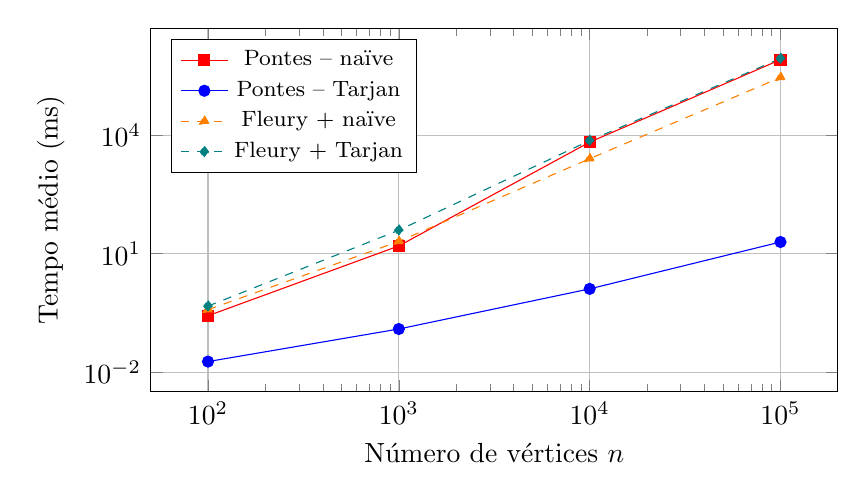
\begin{tikzpicture}
\begin{loglogaxis}[width=0.85\textwidth, height=6.2cm, xlabel={Número de vértices $n$}, ylabel={Tempo médio (ms)}, grid=major, legend pos=north west, legend style={font=\footnotesize}, xtick={100,1000,10000,100000}]
\addplot[color=red, mark=square*] coordinates {(100,0.26809) (1000,15.8007) (10000,6756.98) (100000,832585)};
\addlegendentry{Pontes -- naïve}
\addplot[color=blue, mark=*] coordinates {(100,0.01849) (1000,0.12373) (10000,1.28687) (100000,19.8658)};
\addlegendentry{Pontes -- Tarjan}
\addplot[color=orange, mark=triangle*, dashed] coordinates {(100,0.38273) (1000,20.5541) (10000,2568.21) (100000,294380)};
\addlegendentry{Fleury + naïve}
\addplot[color=teal, mark=diamond*, dashed] coordinates {(100,0.47039) (1000,39.556) (10000,7390.7) (100000,889606)};
\addlegendentry{Fleury + Tarjan}
\end{loglogaxis}
\end{tikzpicture}
\caption{Tempo médio em escala log-log -- grafos da classe euleriano.}
\label{fig:euleriano}
\end{figure}

\begin{figure}[H]
\centering
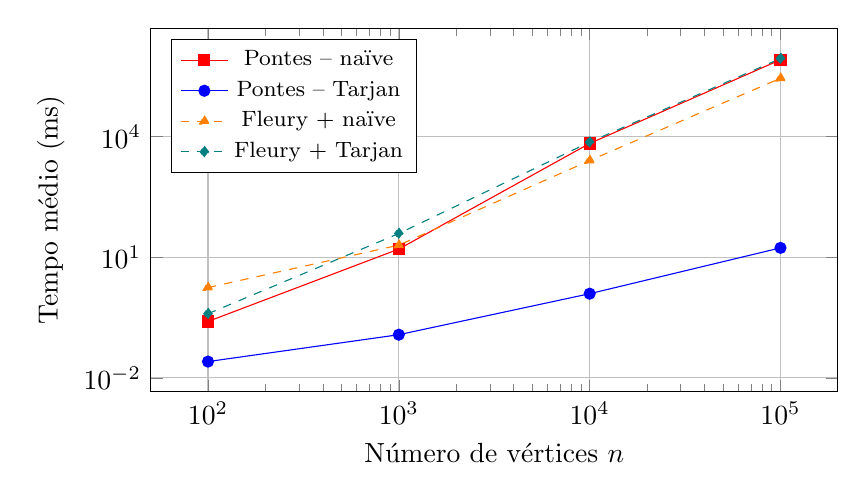
\begin{tikzpicture}
\begin{loglogaxis}[width=0.85\textwidth, height=6.2cm, xlabel={Número de vértices $n$}, ylabel={Tempo médio (ms)}, grid=major, legend pos=north west, legend style={font=\footnotesize}, xtick={100,1000,10000,100000}]
\addplot[color=red, mark=square*] coordinates {(100,0.25368) (1000,16.0522) (10000,6816.04) (100000,822728)};
\addlegendentry{Pontes -- naïve}
\addplot[color=blue, mark=*] coordinates {(100,0.02549) (1000,0.11882) (10000,1.244) (100000,17.183)};
\addlegendentry{Pontes -- Tarjan}
\addplot[color=orange, mark=triangle*, dashed] coordinates {(100,1.76888) (1000,20.125) (10000,2561.79) (100000,285468)};
\addlegendentry{Fleury + naïve}
\addplot[color=teal, mark=diamond*, dashed] coordinates {(100,0.39473) (1000,39.1314) (10000,7347.59) (100000,882548)};
\addlegendentry{Fleury + Tarjan}
\end{loglogaxis}
\end{tikzpicture}
\caption{Tempo médio em escala log-log -- grafos da classe semi-euleriano.}
\label{fig:semi-euleriano}
\end{figure}

\begin{figure}[H]
\centering
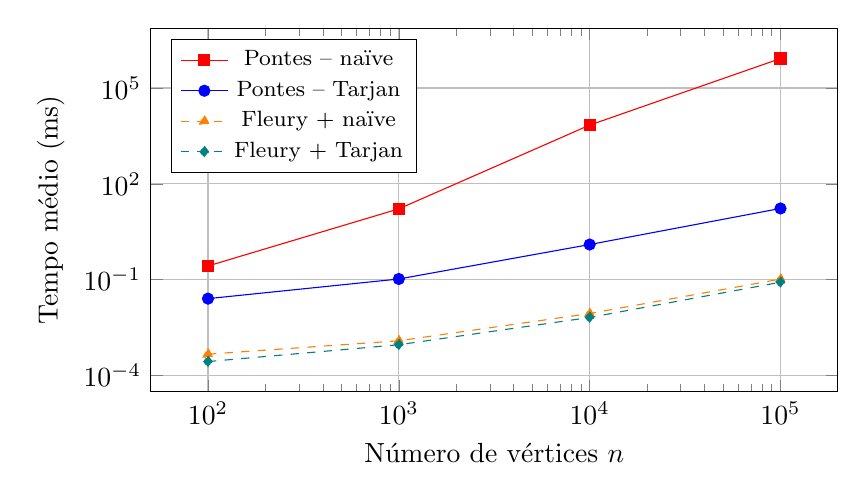
\begin{tikzpicture}
\begin{loglogaxis}[width=0.85\textwidth, height=6.2cm, xlabel={Número de vértices $n$}, ylabel={Tempo médio (ms)}, grid=major, legend pos=north west, legend style={font=\footnotesize}, xtick={100,1000,10000,100000}]
\addplot[color=red, mark=square*] coordinates {(100,0.26641) (1000,16.407) (10000,6883.65) (100000,837576)};
\addlegendentry{Pontes -- naïve}
\addplot[color=blue, mark=*] coordinates {(100,0.02527) (1000,0.10424) (10000,1.25067) (100000,16.8857)};
\addlegendentry{Pontes -- Tarjan}
\addplot[color=orange, mark=triangle*, dashed] coordinates {(100,0.00046) (1000,0.00121) (10000,0.00863333) (100000,0.1032)};
\addlegendentry{Fleury + naïve}
\addplot[color=teal, mark=diamond*, dashed] coordinates {(100,0.00027) (1000,0.00091) (10000,0.0065) (100000,0.0826)};
\addlegendentry{Fleury + Tarjan}
\end{loglogaxis}
\end{tikzpicture}
\caption{Tempo médio em escala log-log -- grafos da classe não euleriano.}
\label{fig:nao-euleriano}
\end{figure}
